\setRL
\pagenumbering{arabic} 


\section{\label{sec:cellmembrane}
غشای سلولی
}
\begin{figure}[h]
\begin{center}
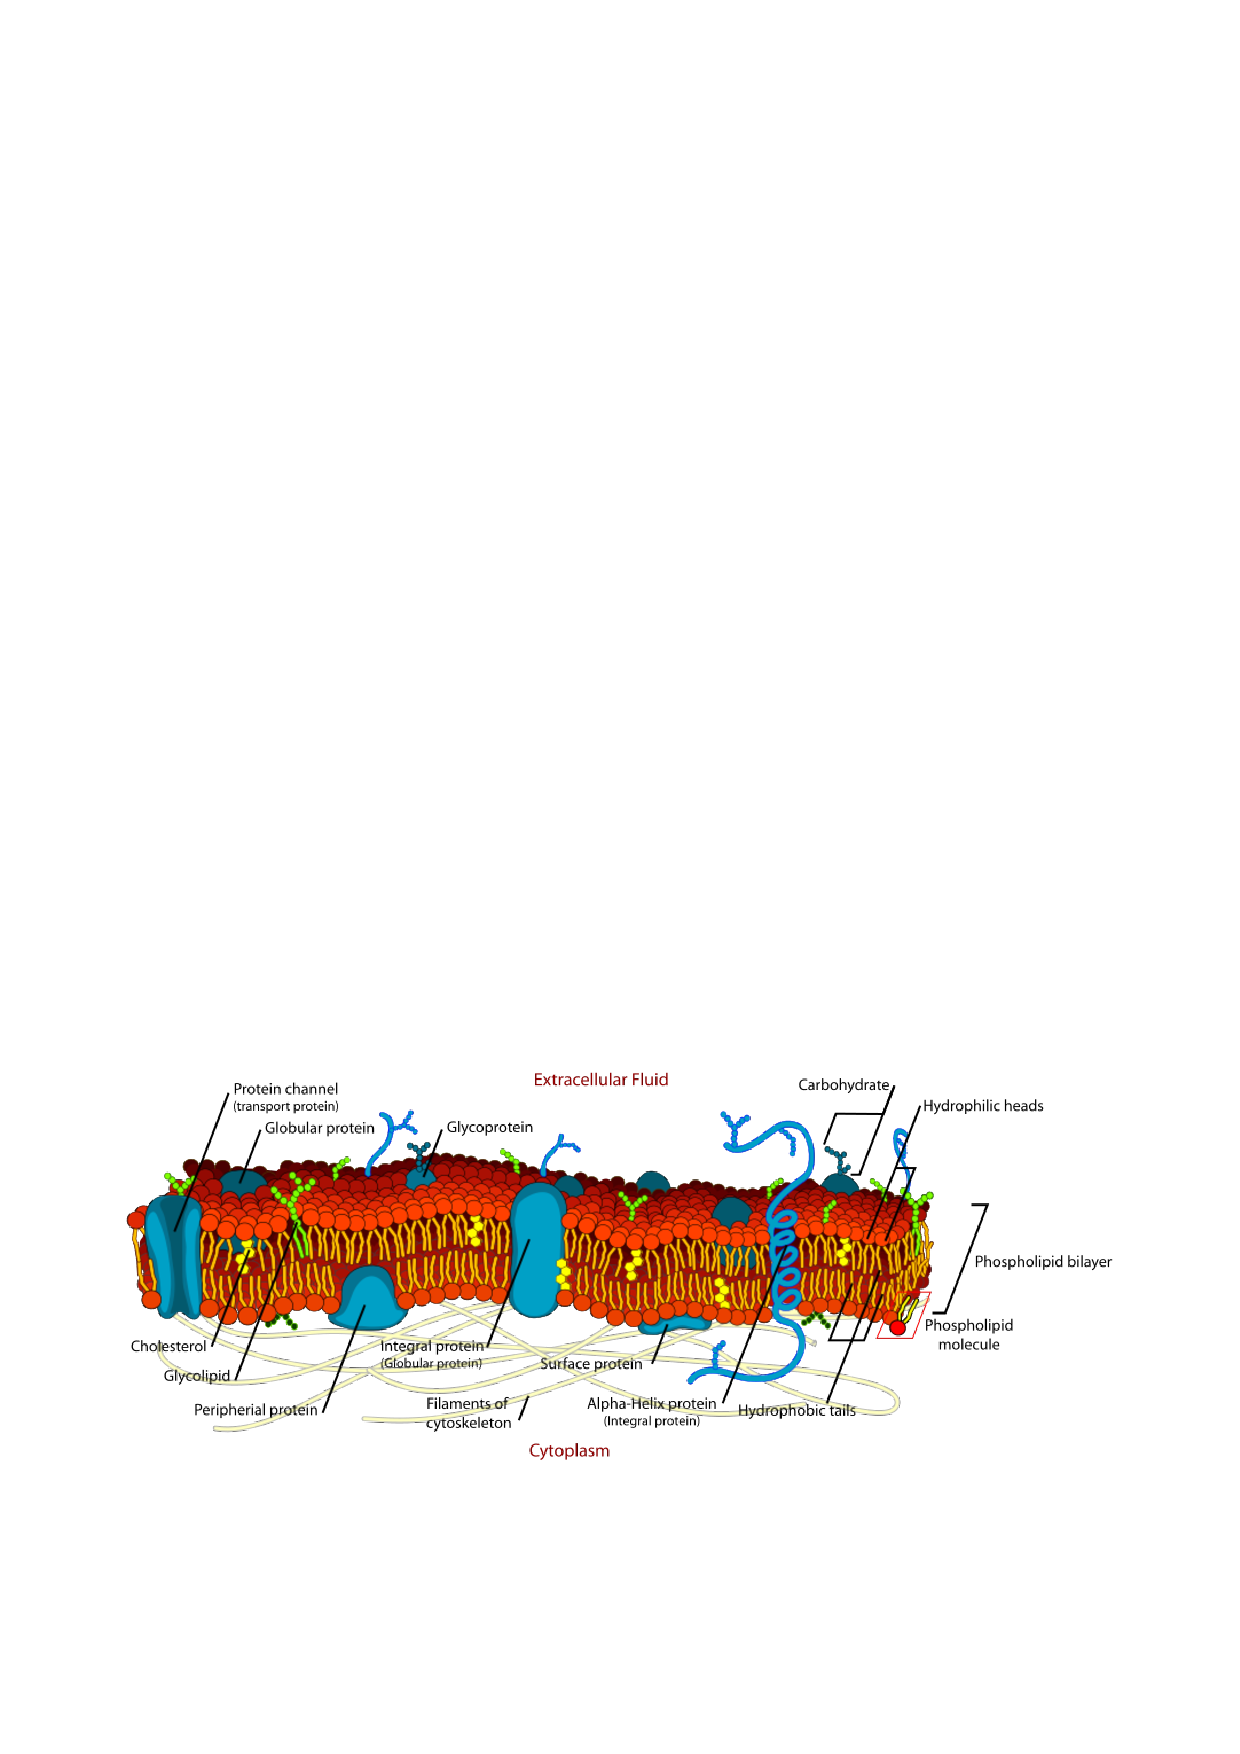
\includegraphics[width=4in]{\MemBio /Pics/Cell_membrane_detailed_diagram}
\caption{
شکل از سایت ویکیپیدیا گرفته شده است
\cite{wikiCellMembrane}
. نقاشی غشا بر اساس مدل غشای مایع موزایکی است. بیشتر غشا از ملکول‌های چربی تشکیل شده ولی پروتئین‌های خیلی زیادی در غشا قرار دارند. همچنین غشا از طریق این پروتئین‌ها به اسکلت سلولی و اجزای دیگر متصل است. دایره‌های قرمز سر آب دوست و رشته‌های زرد دم‌های آب گریز لیپید‌ها را نشان می‌دهد.
}
\label{fig:fluidmembranemodel}
\end{center}
\end{figure}

زحمات افراد در قرن ۱۹ و ۲۰ میلادی برای پی بردن به ساز و کار واحد‌های سازنده‌ی موجودات زنده، تصویری پر از جزئیات از سلول زنده ساخته است. در سال ۱۹۸۵ ارنست اُورتن 
\LTRfootnote{Ernest Overton}  
سلول‌های گیاهی را در محلول‌های مختلف (قند،‌ الکل، اتر، فنول، و استن
\LTRfootnote{sugar, alcohols, ether, phenol, and acetone}
) قرار داد. مشاهدات وی نشان داد که (تحت اختلاف فشار اسمزی یکسان) محلول‌هایی مانند قند که در آب به راحتی حل می‌شوند نمی‌توانند وارد سلول شوند در صورتی که محلول‌هایی که در آب حل شوندگی خوبی ندارند، می‌توانند وارد سلول شوند. او نتیجه گرفت که جنس مرز سلول با سیتوپلاسم درون آن متفاوت است و به احتمال زیاد از ملکول‌های چربی گون تشکیل شده است
\cite{overton1985}
. در سال ۱۹۳۲ (حدود صد سال پیش) کِنِت کول
 \LTRfootnote{Kenneth Cole}
 تخم جوجه‌تیغی دریایی
 \LTRfootnote{sea urchin (arbacia) egg} 
 را با یک فیبر از جنس طلا بر روی یک سطح فشار داد. با اندازه گیری  کشش سطحی و حد تحمل فشار تخم، استدلال کرد که لایه‌ی نازک اطراف سلول فقط از ملکول‌های چربی درست نشده است
 \cite{Cole1932}
. در دهه‌ی ۱۹۵۰ با تکنولوژی میکروسکوپ الکترونی، اولین تصاویر از غشای سلول رونمایی شد و با استفاده از روش‌های رنگ آمیزی، وجود لیپید‌ها
\LTRfootnote{lipid}
 در غشا تایید شد. 
ضخامت غشای سلولی بین ۵ تا ۱۰ نانومتر اندازه‌گیری شد
\cite{ROBERTSON1959aa}
. افراد زیادی در تکمیل‌ کردن تصویر غشای سلول  نقش داشتند، ولی تصویر مدرنی که ما از غشاهای سلول‌ها زنده داریم بیشتر بر پایه‌ی مدل غشای مایع موزایکی‌
\LTRfootnote{the mosaic fluid model of membranes}
 است که در سال ۱۹۷۲ توسط سینگر
 \LTRfootnote{Singer}
  و نیکلسون
  \LTRfootnote{Nicholson}
 ارائه شد
\cite{Singer1972}
(شکل 
\ref{fig:fluidmembranemodel}
). بنا بر این مدل غشا را می‌توان یک مایع دو بعدی فرض کرد که در آن چربی‌ها و پروتئین‌ها می‌توانند کم و بیش آزادانه حرکت کنند. در نتیجه هیچ نظم بلند بردی در غشا دیده نمی‌شود. با وجود اینکه غشای چربی به طور خود سامانده تشکیل می‌شود ولی علاوه بر آن پروتئین‌های زیادی نیز وجود دارد که به غشا ساختار می‌بخشند
\cite{wikiCellMembrane}
. غشا از طریق این پروتئین‌ها به اجزای پیچیده‌تر داخل سلول (مانند اسکلت سلولی) متصل است. خاصیت تراوایی فوسفولیپید دو لایه و کانال‌های پروتئینی درون غشا، ارتباط سلول با محیط اطراف را کنترل و مدیریت می‌کند. 







 
 \begin{figure}[h]
\begin{center}
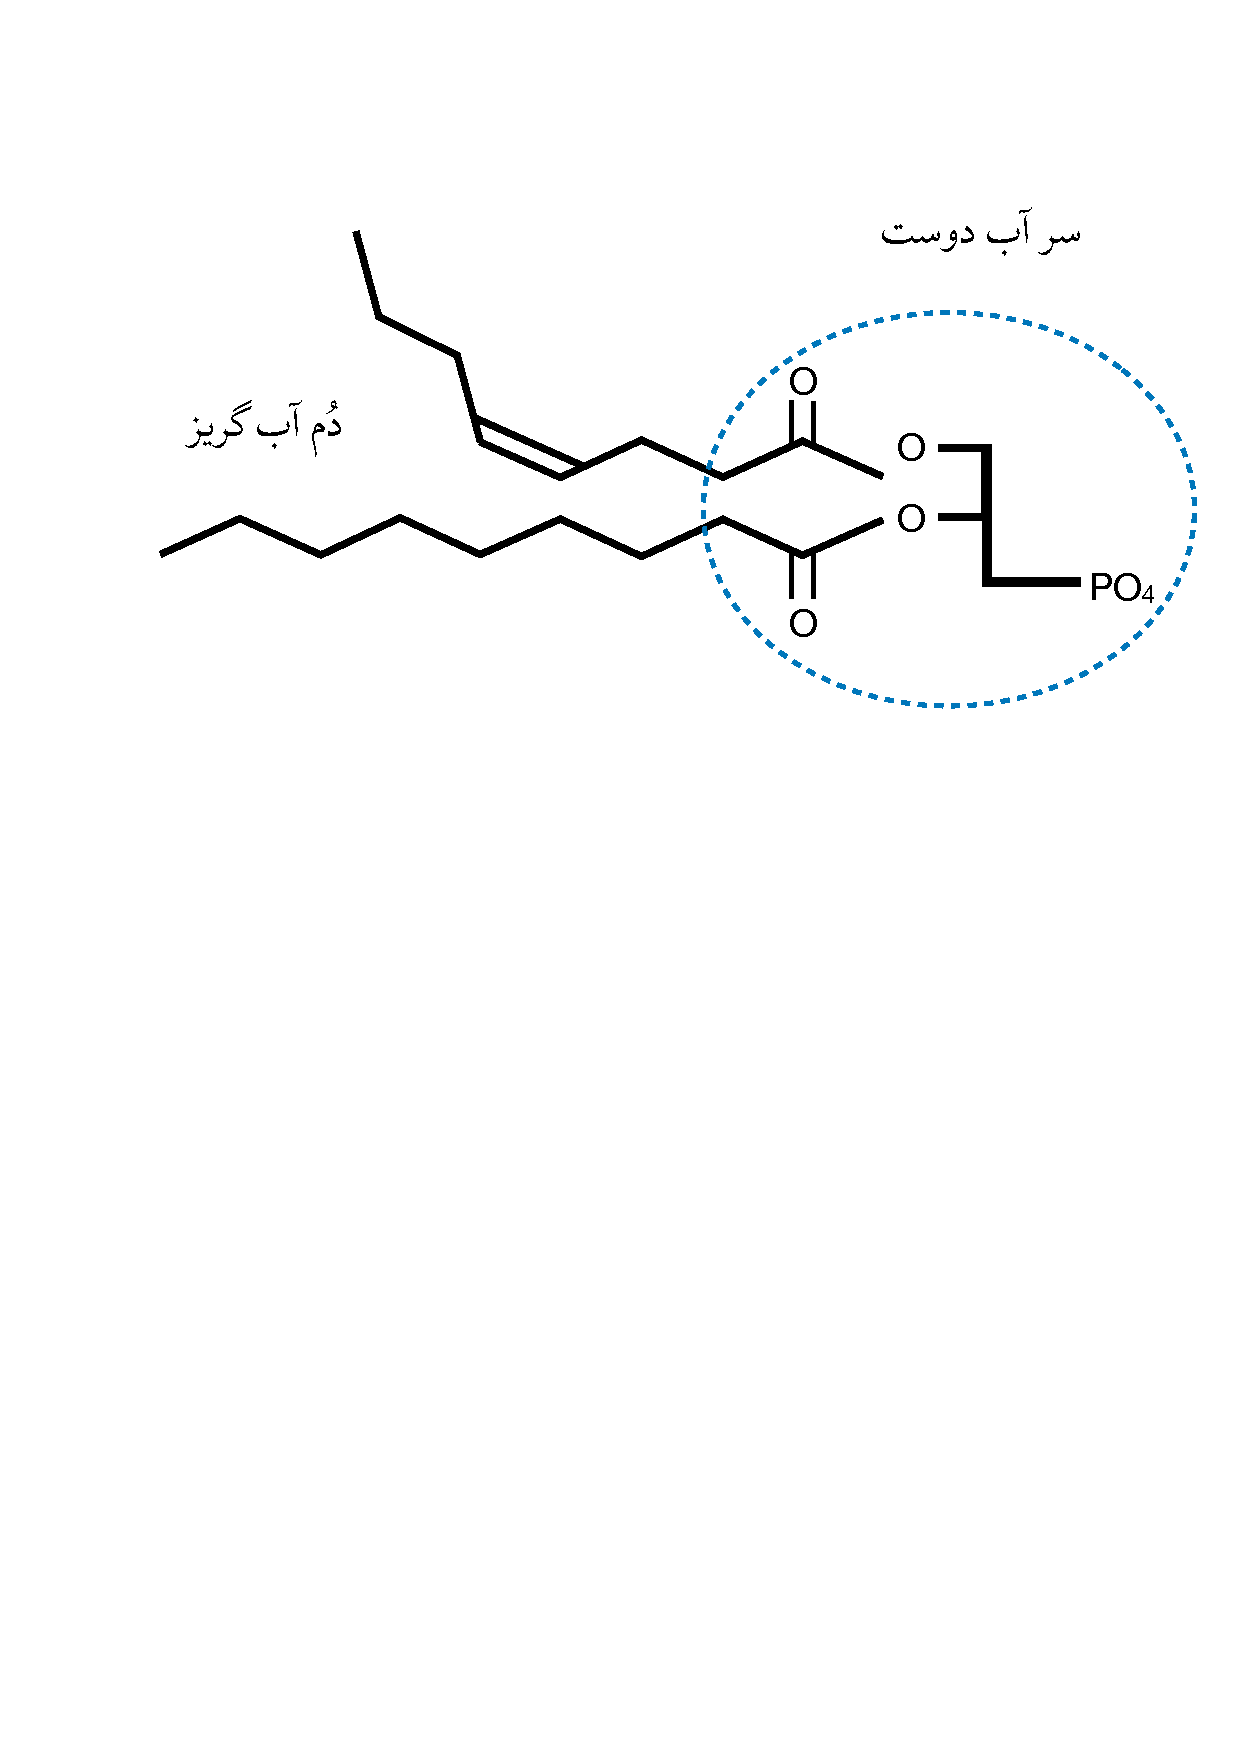
\includegraphics[width=4in]{\MemBio /Pics/Phospholipid}
\caption{
ساختار شیمیایی یک ملکول فوسفولیپید. سر آب دوست (دایره‌ی آبی) و  انتهای آبگریز مشخص شده است.
}
\label{fig:phospholipid}
\end{center}
\end{figure}
 
 
 ملکول‌های فوسفولیپید از یک سر آب دوست
\LTRfootnote{hydrophilic}  
 و یک دُم آب گریز
 \LTRfootnote{hydrophobic}  
 ساخته شده‌است (شکل
\ref{fig:phospholipid}
). وجود این دو سر باعث می‌شود که این ملکول‌ها در محلول‌های آبی
\textbf{بدون ایجاد پیوندها شیمیایی}
، به طور خود سامانده
  \LTRfootnote{self-assembly}  
 سطوح بزرگ دولایه تشکیل دهند.  دُم‌های  آبگریز در مرکز لایه (به دور از آب) و سر آب دوست به سمت محلول جهت‌گیری می‌کنند (شکل
\ref{fig:bilayer}
 ).
\begin{figure}[h]
\begin{center}
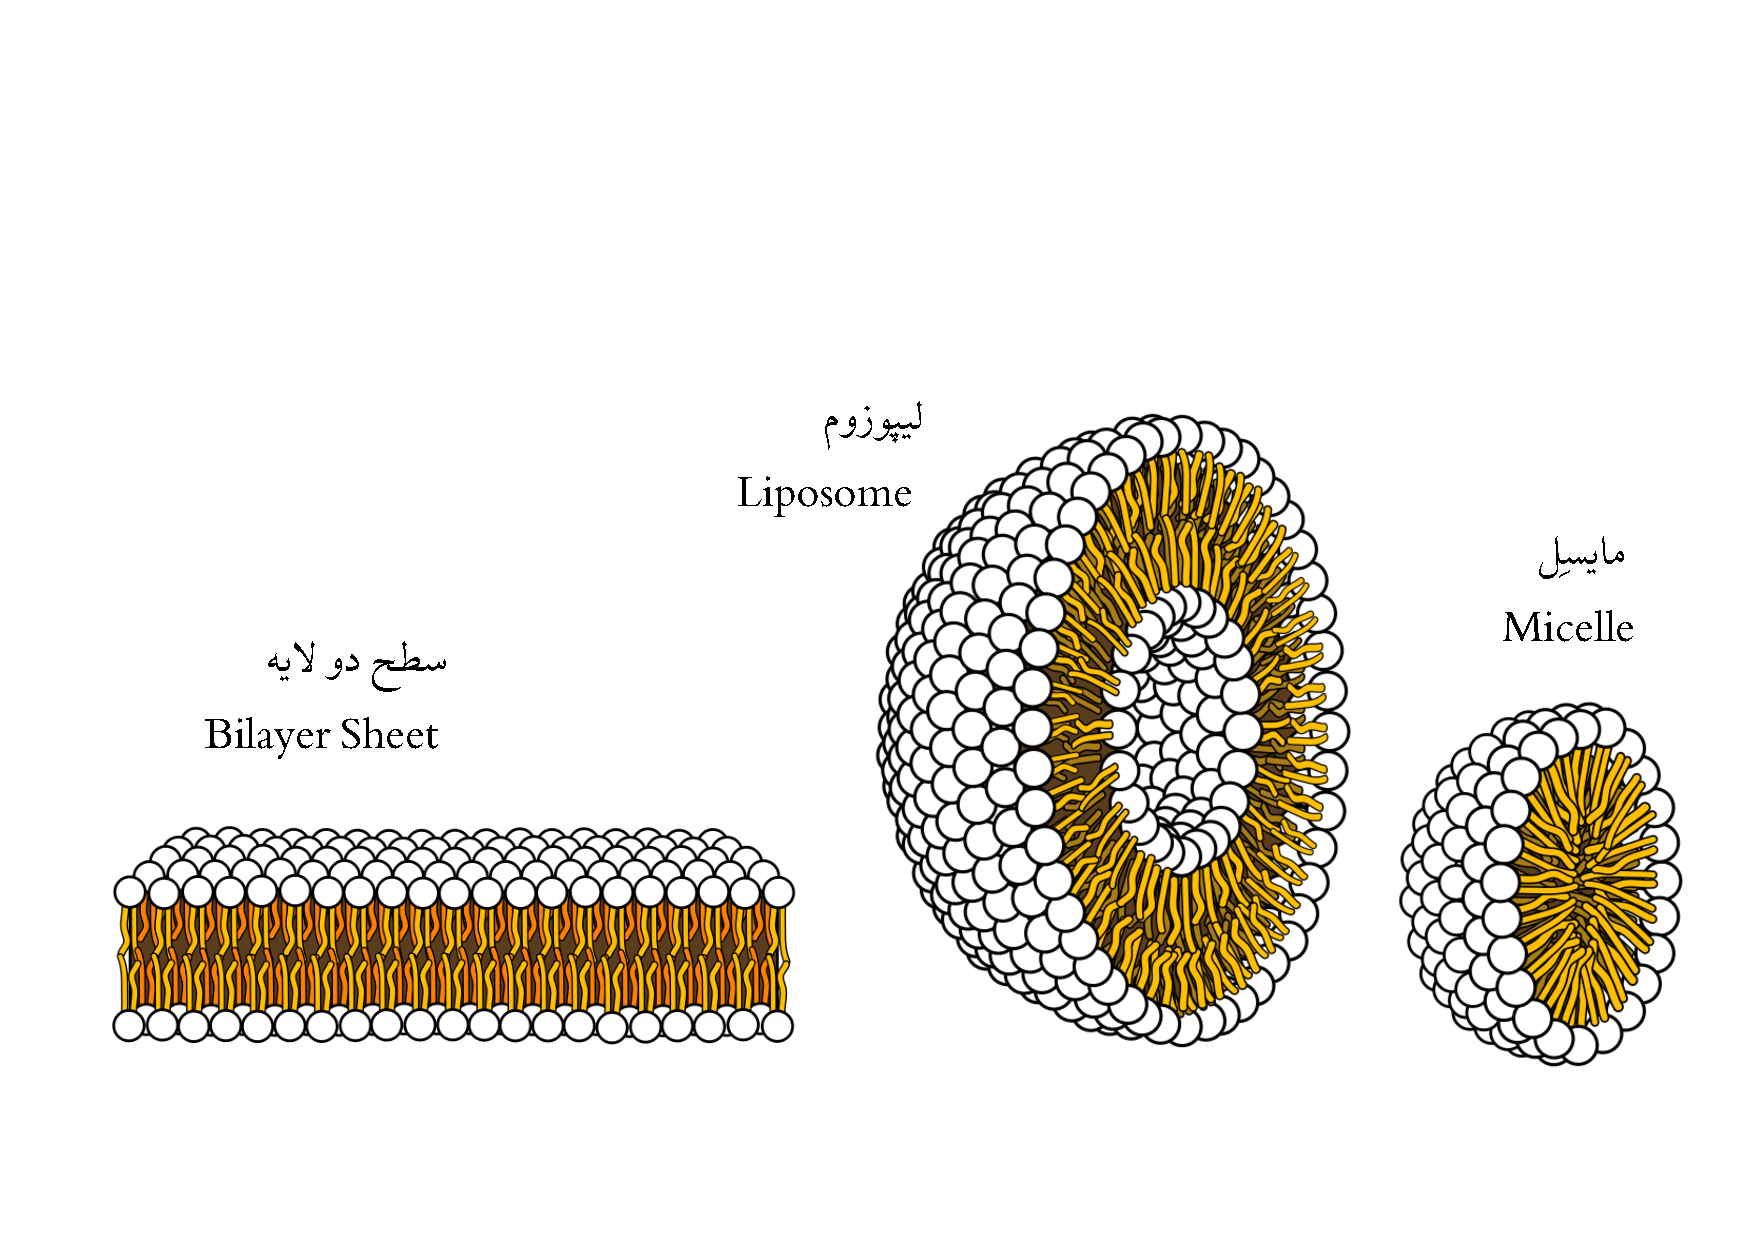
\includegraphics[width=4in]{\MemBio /Pics/Bilayer}
\caption{
ساختار‌های معمول ملکول‌های چربی در آب. به ترتیب از چپ به راست، ساختار سطوح بزرگ دو لایه، کره‌های دو لایه (لیپوزوم)، و کره‌های کوچک تک لایه، مایسِل.
}
\label{fig:bilayer}
\end{center}
\end{figure}
البته با گسترش تحقیقات ما می‌دانیم غشا‌های زیستی بیشتر شکل موزائیکی دارند تا مایع. غشاها موزائیکی هستند به این معنی که در سلول‌های مختلف غشا خیلی همگن نیست و در سلول‌ها قسمت‌هایی از غشا دیده‌ می‌شود که ترکیب پروتئینی متفاوتی از بخش‌های دیگر داشته باشند و یا ضخامت برخی از بخش‌های غشا ممکن است از چند ۱۰ نانومتر تا ۱۰۰ نانومتر تغییر کند
\cite{Engelman:2005aa}
.
 
 
 
 
 
 
 
 
 
 
 
 
 
 
 